\subsection{Using ssu-build to create a truncated model of a specific region of SSU rRNA}
\label{sec:tutorial-build-v4}

Many SSU sequencing studies target a specific region of the SSU rRNA
molecule using PCR primers at the boundaries of that region.  For such
studies, you may want to build a new CM that only models the
region of the molecule targeted by the study.
There are two reasons for doing this. The first is speed: the
running time of \prog{ssu-align} decreases as the model size it is
using decreases (see table~\ref{tbl:ttimes} on
page~\pageref{tbl:ttimes} and the associated text in
section~\ref{sec:stats}). The second reason is that 
it should slightly increase alignment accuracy because the uncertainty 
regarding what region of the full molecule the subsequence should
align to is eliminated \footnote{Though
  recommended, building truncated models for PCR studies is not
  required. \prog{ssu-align} is designed to be able to handle
  truncated sequences deriving from any region of the SSU molecule}.
In this section I'll demonstrate how to create a CM of a
specific region of SSU and use it to create alignments.

In this example, we'll build three new CMs targetted to the so-called
V4 hypervariable region, one each for archaea, bacteria and
eukarya. We'll do this using the SSU-ALIGN default seed
alignments that were used to create the default full-length CMs.

The first step is to identify the region of each of the three default
models we want our new models to represent. The secondary structure
diagrams in the \prog{models/} subdirectory of the
\prog{ssu-align-0.1.1/} toplevel directory where you unpacked the package.
In particular, the files suffixed with \prog{.rf.pdf} and
\prog{.info.pdf} are probably most useful. These figures are included
in this guide in section~\ref{sec:models} as
figures~\ref{fig:arcrf} and \ref{fig:arcinfo} (archaea),
\ref{fig:bacrf} and \ref{fig:bacinfo} (bacteria),
\ref{fig:eukrf} and \ref{fig:eukinfo} (eukarya).
In these figures, every 100th position is numbered, and every 10th
position is indicated by a tick mark.

Based on the bacterial primer sites used by a recent environmental
study that targetted the V4 region \cite{Claesson09}, I determined 
the V4 region in the default bacterial model spans positions 584
through 824 via manual inspection of the bacterial secondary structure
diagrams. By comparison to the archaeal and eukaryal diagrams, 
the corresponding region in archaea is from positions 525 to
765, and in eukarya is 620 to 1082. 

Given these coordinates, we can use \prog{ssu-build} to create V4
specific models. 
First, create and move into a new directory where we'll build the new
models. For example, from the \prog{tutorial/} directory, do:

\user{mkdir myV4; cd myV4}

The models must be built one at a time. First, we'll
create the archaeal V4 model:

\user{ssu-build -d --trunc 525-765 -n arc-V4 -o V4.cm archaea}

The \prog{-d} option tells \prog{ssu-build} to use a default model,
\prog{--trunc 525-765} specifies the positions of the model, \prog{-n arc-V4}
specifies the name of the model should be \prog{arc-V4} and \prog{-o
  V4.cm} specifies the name of the CM file be \prog{V4.cm} (we'll add
two more models to this file next). Finally, \prog{archaea} tells the
program to use the default archaeal model. As with the other programs,
\prog{ssu-build} reports on what it's doing:

\begin{sreoutput}
# Truncating alignment and default mask; saving only columns between predefined consensus
# columns 525 and 765...
#
# output aln file           
# --------------------------
  archaea-0p1-sb.525-765.stk
#
# truncated mask file name   
# ---------------------------
  archaea-0p1-sb.525-765.mask
#
# Building CM(s)...
#
#                           num  alignment  consensus   num
# CM file name  CM name    seqs     length     length   bps
# ------------  -------  ------  ---------  ---------  ----
  V4.cm         arc-V4       23        242        241    69
#
# structure diagram file    
# --------------------------
  archaea-0p1-sb.525-765.pdf
#
\end{sreoutput}


Several files have been created as listed below:

\begin{sreitems}{}

\item[\prog{archaea-0p1-sb.525-765.stk}] the region of the default
  archaeal seed alignment spanning consensus columns 525 to
  765. This alignment was used to build the new archaeal V4 model.
  
\item[\prog{archaea-0p1-sb.525-765.mask}] the region of the default
  archaeal mask (see section~\ref{sec:masks}) spanning consensus
  columns 525 to 765. This mask file could potentially be useful to mask
  alignments created using the new archaeal V4 model with the
  \prog{ssu-mask} option and the \prog{-s} option.
  
\item[\prog{V4.cm}] the CM file with the new archaeal V4 model named
  \prog{arc-V4}. As indicated by the output, the model was built
  from an alignment of width 242 positions that included 69
  basepairs of 23 archaeal sequences. This alignment was saved as
  \prog{archaea-0p1-sb.525-765.stk}.
  
\item[\prog{archaea-0p1-sb.525-765.ps}] a structure diagram 
  of the archaeal consensus model highlighting the region from
  positions 525 to 765 represented by the new model in \prog{V4.cm}.
  This diagram is included as figure~\ref{fig:V4}.
\end{sreitems}

Next we'll build bacterial V4 and eukaryal V4 models and append them
to the \prog{V4.cm} file:

\user{ssu-build -d --trunc 584-824 -n bac-V4 --append V4.cm bacteria}

\user{ssu-build -d --trunc 620-1082 -n euk-V4 --append V4.cm eukarya}

The \prog{--append} option tells \prog{ssu-build} to append the new model
onto the existing file \prog{V4.cm}.
After executing these two commands, the \prog{V4.cm} file will contain
three V4 models. This CM file can be used to create domain-specific
SSU V4 alignments from a set of SSU sequences using
\prog{ssu-align}. An example dataset this would be particularly useful
for would be a set of SSU sequences generated from an environmental
sequencing survey that used three sets of PCR primers: one each for
the archaeal, bacterial and eukaryal V4 regions. Alternatively, it
could be used to create V4-only alignments from a set of full length
SSU sequences. We'll demonstrate the latter application here using our
sample dataset from earlier in the tutorial in the file:
\prog{tutorial/seed-15.fa}, which contains 15 full or nearly-full
length archaeal, bacterial and eukaryotic SSU sequences:

\user{ssu-align -m V4.cm ../seed-15.fa myV4seqs}\footnote{This assumes your
  current working directory is in a subdirectory of \prog{tutorial/}.
  If not, specify the correct path to the \prog{seed-15.fa} file
  in the \prog{tutorial/} subdirectory of \prog{ssu-align-0.1.1/}.}

The \prog{-m} option specifies that the model \prog{V4.cm} be used. 
Using this model, processing \prog{seed-15.fa} takes only about 4
seconds, as opposed to the 30 seconds it took with the default,
full-length models earlier in the tutorial. Take a look at
\prog{myV4seqs/myV4seqs.bacteria.stk}, it contains only the V4 regions
of the 5 bacterial sequences from \prog{seed-15.fa}. 

As with the earlier example, these alignments can be masked with the
\prog{ssu-mask} program, though I won't step through that
here. However, the \prog{ssu-draw} program cannot be used to draw
diagrams of alignments created using any models other than the default
three, so it is not possible to create drawings of these alignments.


\begin{sidewaysfigure}
  \begin{center}
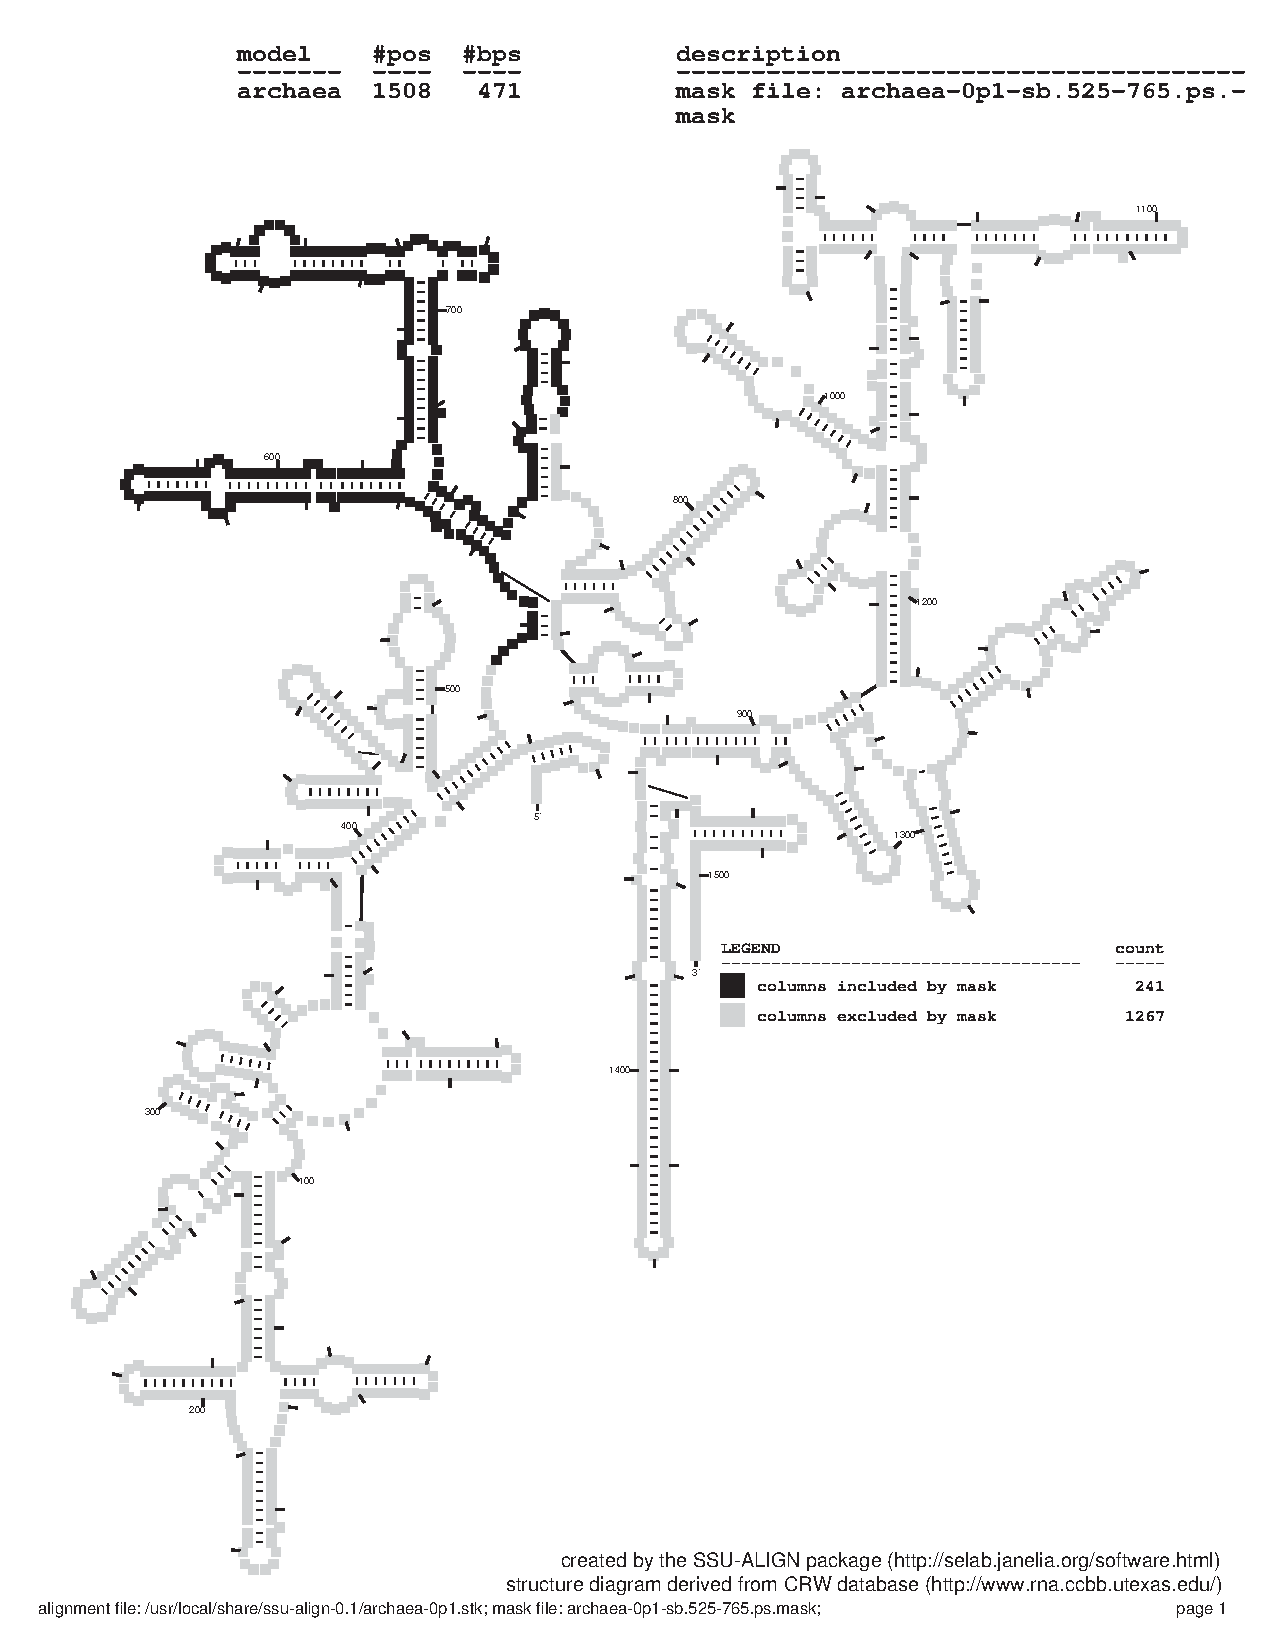
\includegraphics[width=2.8in]{Figures/arc-v4}
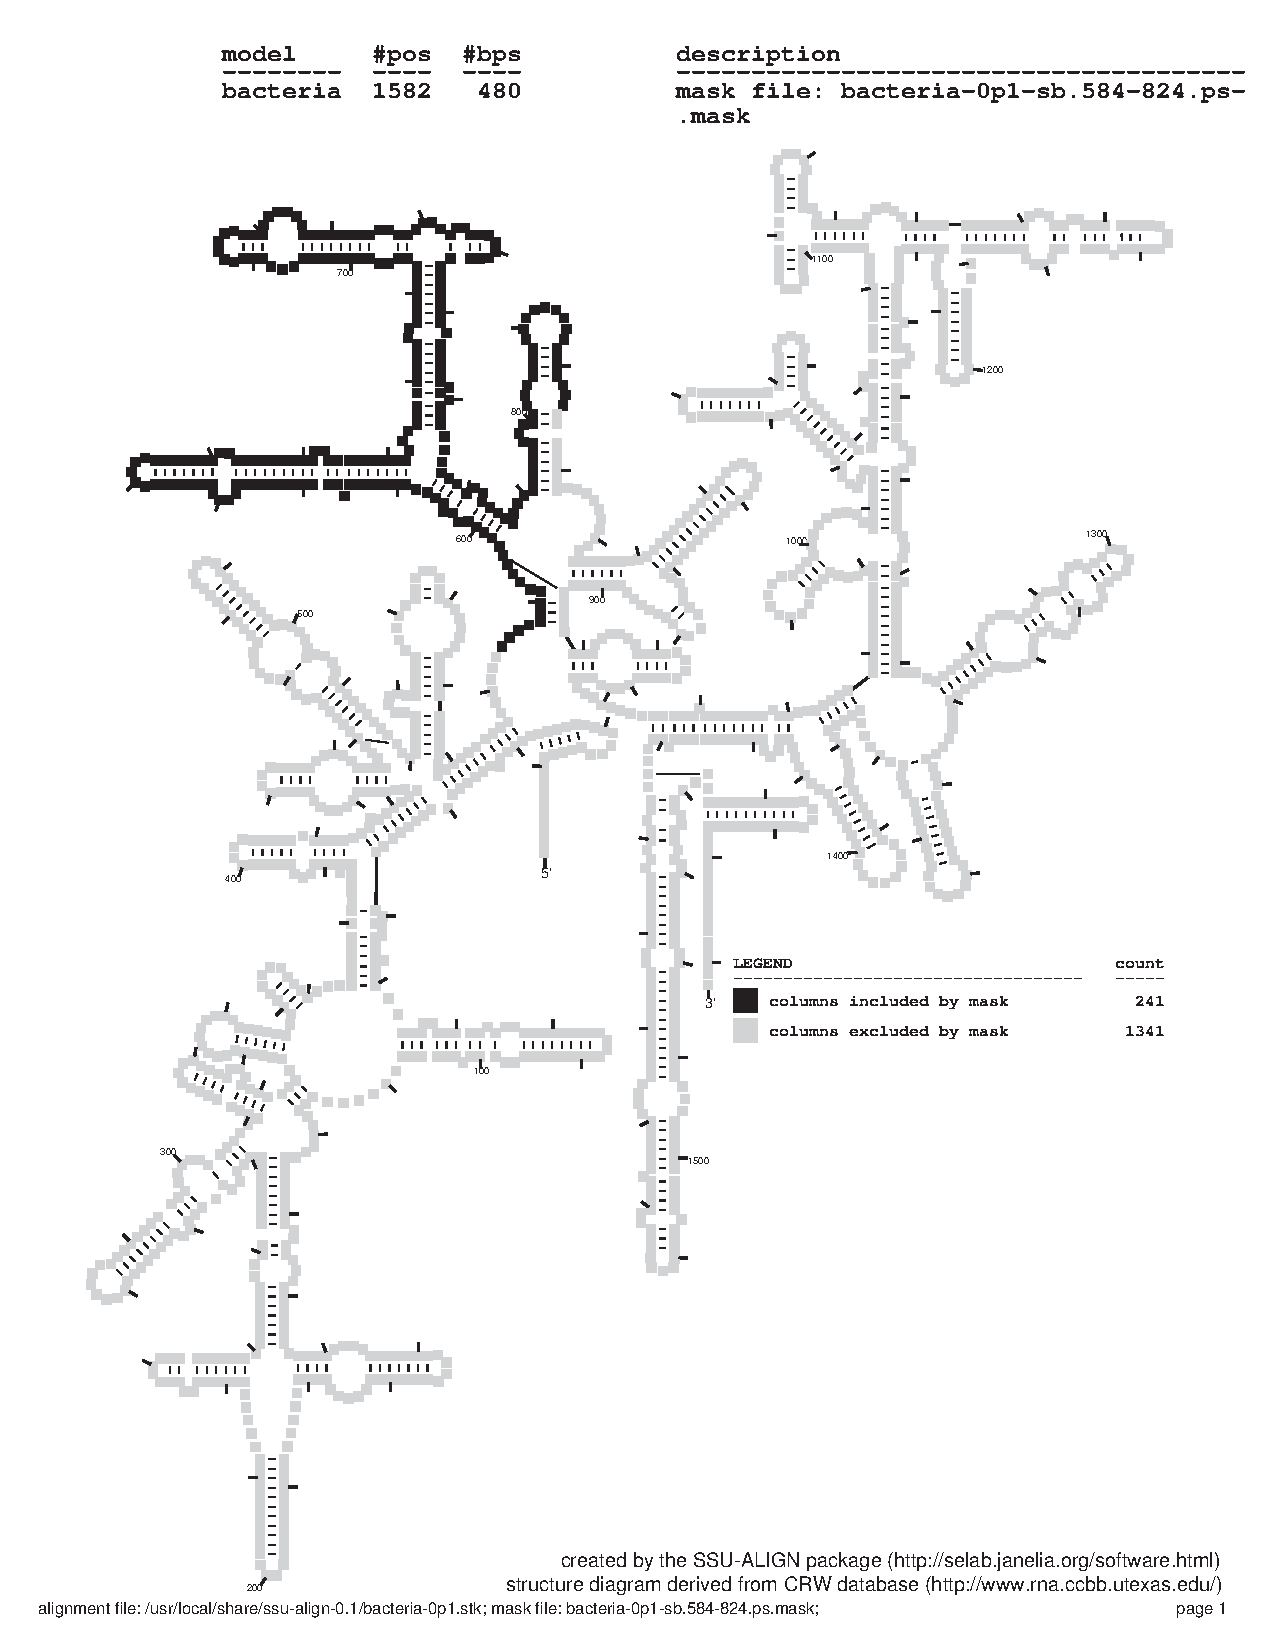
\includegraphics[width=2.8in]{Figures/bac-v4}
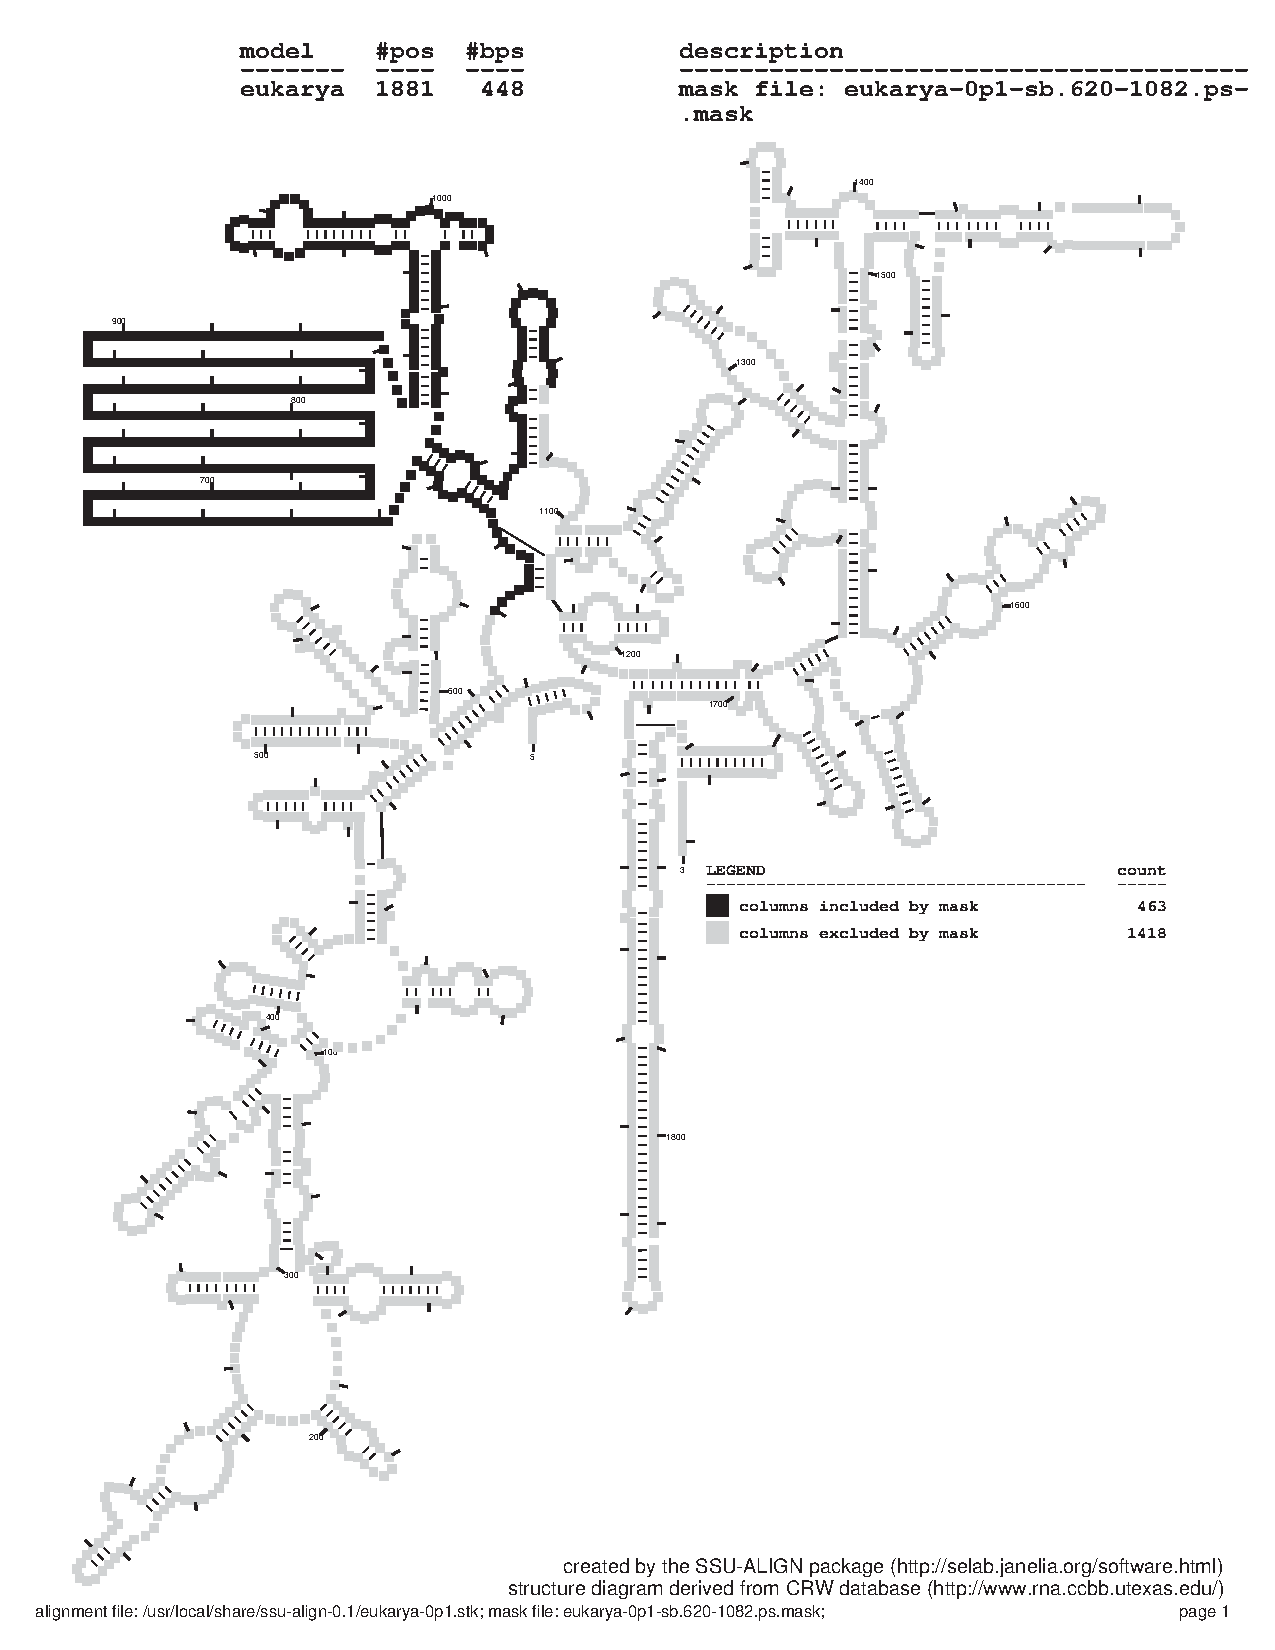
\includegraphics[width=2.8in]{Figures/euk-v4}
  \end{center}
\caption{\textbf{V4 regions in archaea (left), bacterial (middle) and eukarya
  (right).} These diagrams are generated by \prog{ssu-build} in the
  tutorial.}
\label{fig:V4}
\end{sidewaysfigure}
